\section{Detector signals}\label{sec:1.5}

A detector records none of the dark-matter flux (\cref{sec:1.2}), the energy and momentum it can transfer (\cref{sec:1.3}) or the strength of its interaction (\cref{sec:1.4}) directly. It counts quanta: electrons, phonons, quasiparticles or photons produced as the deposited energy relaxes. We will follow the energy from the deposit to the quanta a sensor counts, assemble the event rate, and turn a count of events into a limit on $\sigmae$. \Cref{fig:1-chain} shows the chain that the rest of the book follows.

\begin{figure}[tbp]
  \centering
  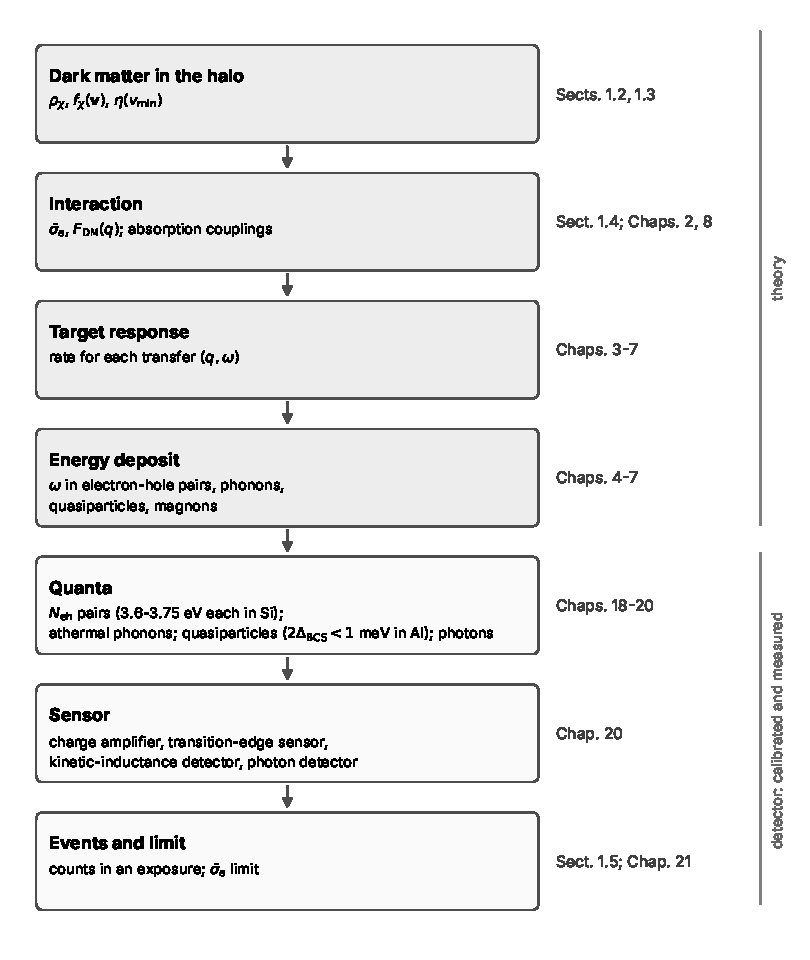
\includegraphics[width=0.78\linewidth]{figures/ch01/fig1_8.pdf}
  \caption{The signal chain from dark matter to sensor. The upper four steps are computed from theory: the halo (\cref{sec:1.2,sec:1.3}), the interaction (\cref{sec:1.4}; \cref{chap:2,chap:8}), the target response and the primary excitations (\cref{chap:3,chap:4,chap:5,chap:6,chap:7}). The lower three are fixed by calibration and measurement: the conversion of the deposit into countable quanta (\cref{chap:18,chap:20}), the sensor (\cref{chap:20}) and the statistical step from counts to a limit (\cref{sec:1.5}; \cref{chap:21}). Energies per quantum are from Refs.~\cites[Table~I]{ramanathan2020ionization}[Sect.~2.2.1]{hochberg2016detecting}.}
  \label{fig:1-chain}
\end{figure}

\subsection{Readout quanta}\label{sec:1.5-quanta}

A deposit of a few eV or less does not stay in the excitation that the dark matter created. Hot electrons and holes lose energy to further electron--hole pairs and to phonons; quasiparticles in a superconductor emit phonons; phonons decay into lower-energy phonons. Detectors read the products at one of four stages: as charge, as heat carried by phonons, as quasiparticles of a superconductor, or as photons~\cite[Sect.~VII]{kahn2022searches}. Each channel counts a different quantum, and the energy per quantum sets how finely a deposit is resolved.

\paragraph{Charge.} In a semiconductor an excitation across the band gap promotes an electron to the conduction band and leaves a vacancy, a \emph{hole}, in the valence band. The pair is called an \emph{electron--hole pair}. Both carriers are mobile, and an applied electric field drifts them to electrodes before they recombine~\cite[Sect.~VII\,A]{kahn2022searches}. The number of pairs produced by a deposit $\omega$ is the \emph{ionization yield} $N_{\mathrm{eh}}$. A primary carrier with energy well above the gap creates further pairs by impact ionization, knocking further electrons across the gap, and also emits phonons; on average, then, each pair costs more than $\Eg$. For deposits well above \SI{20}{eV} the mean yield is proportional to the deposit~\cite[abstract and Eq.~(1)]{ramanathan2020ionization},
\begin{equation}
  \langle N_{\mathrm{eh}}\rangle = \frac{\omega}{\varepsilon_{\mathrm{eh}}} ,
  \label{eq:1.5-yield}
\end{equation}
with the mean energy per pair $\varepsilon_{\mathrm{eh}}$. Measurements in silicon give \SIrange{3.62}{3.66}{eV} at \SI{300}{K} and \SIrange{3.70}{3.75}{eV} between \SI{5}{K} and \SI{123}{K}~\cite[Table~I]{ramanathan2020ionization}, roughly three times the gap. The excess goes into phonons. The fluctuations of $N_{\mathrm{eh}}$ are smaller than Poisson fluctuations: the variance is 0.1 to 0.15 times the mean~\cite[Eq.~(5.4)]{essig2016direct}. A \SI{100}{eV} deposit produces on average $100/3.7 = 27$ pairs with a spread of $(0.12 \times 27)^{1/2} = 1.8$, against $27^{1/2} = 5.2$ for a Poisson count. The pairs are not produced independently: the energy is fixed, and a cascade that makes one more pair has less energy left for the next.

Light dark matter, however, deposits only a few eV, where \cref{eq:1.5-yield} fails. Below $2\Eg$ energy conservation allows one pair at most; between that and a few tens of eV the yield depends on how the primary carriers share the energy, and the silicon data cover 3 to \SI{8}{eV} and then \SI{50}{eV} upward, with nothing in between~\cite[Sect.~III]{ramanathan2020ionization}. A widely used step model assigns one pair for the first $\Eg$ and one more for each further $\varepsilon_{\mathrm{eh}}$~\cite[Eq.~(5.1)]{essig2016direct},
\begin{equation}
  N_{\mathrm{eh}}(\omega) = 1 + \left\lfloor \frac{\omega - \Eg}{\varepsilon_{\mathrm{eh}}} \right\rfloor \qquad (\omega \ge \Eg),
  \label{eq:1.5-step}
\end{equation}
where $\lfloor x\rfloor$ is the largest integer not above $x$. With the low-temperature gap $\Eg = \SI{1.17}{eV}$ of \cref{we:1-mmin} and $\varepsilon_{\mathrm{eh}} = \SI{3.6}{eV}$~\cite[Eq.~(5.2)]{essig2016direct}, a \SI{5}{eV} deposit makes $1 + \lfloor 1.06\rfloor = 2$ pairs and a \SI{10}{eV} deposit $1 + \lfloor 2.45\rfloor = 3$. \Cref{chap:18} derives the yield from the carrier cascade.

A detector that counts pairs states its threshold as a number of pairs, and \cref{eq:1.5-step} turns that number into an energy. The $n$-th pair appears at $\omega = \Eg + (n-1)\varepsilon_{\mathrm{eh}}$, and thresholds of one, two and three pairs then correspond to 1.17, 4.77 and \SI{8.37}{eV}. Through $m_{\mathrm{min}} = 2E_{\mathrm{th}}/v_{\mathrm{max}}^2$ (\cref{eq:1.3-mmin}) with $v_{\mathrm{max}} = \num{2.650e-3}$, these translate into threshold masses of 0.33, 1.36 and \SI{2.38}{MeV}. A search that discards the single-pair bin, where the dark counts described below accumulate, gives up a factor of four in mass reach for a cleaner sample. Since the yield has not been measured in silicon between 8 and \SI{50}{eV}, the energy assigned to a three-pair threshold, and with it $m_{\mathrm{min}}$, carries a model uncertainty (\cref{sec:1.3-edge}).

Skipper charge-coupled devices and calorimetric detectors count single charges. A skipper charge-coupled device measures the charge in each pixel many times without destroying it; the noise falls with the square root of the number of measurements, below 0.1 electron per pixel~\cite[Sect.~VII\,A]{kahn2022searches}. A calorimetric detector instead drifts the carriers across a bias voltage $V_{\mathrm{bias}}$. Each carrier then emits phonons in proportion to the work done on it (the Neganov--Trofimov--Luke effect). The phonon energy is~\cite[Eq.~(195)]{kahn2022searches}
\begin{equation}
  E_{\mathrm{ph}} = E_{\mathrm{prim}} + N_{\mathrm{eh}}\, e V_{\mathrm{bias}} ,
  \label{eq:1.5-luke}
\end{equation}
where $E_{\mathrm{prim}}$ is the part of the deposit that went directly into phonons, at most $\omega$; the second term is usually much larger.
At $V_{\mathrm{bias}} = \SI{150}{V}$ each pair adds \SI{150}{eV}, and the spectrum shows peaks at integer $N_{\mathrm{eh}}$~\cite[Sect.~VII\,A]{kahn2022searches}. In both devices the lowest bins are polluted by a dark rate, charge that leaks across the gap without any deposit, and single-pair events carry the largest background.

\paragraph{Phonons.} Every excitation of a solid ends as phonons, the quantized lattice vibrations of \cref{sec:1.3}. A calorimeter measures this heat and with it the total deposit, whatever the primary excitation~\cite[Sect.~VII\,B]{kahn2022searches}. The phonons first created in silicon are optical phonons of about \SI{64}{meV}; through several anharmonic decays they eventually become acoustic phonons of a few meV. At an operating temperature of \SI{15}{mK} the thermal phonons carry about \SI{1}{\micro eV}, and the signal phonons are far from equilibrium (\emph{athermal}) and cross the crystal ballistically before they reach a sensor on the surface~\cite[Sect.~VII\,B]{kahn2022searches}. The quanta are too numerous and too soft to count one by one. The sensor integrates their energy, and its noise sets the threshold: a \SI{10.6}{g} silicon crystal read by a tungsten transition-edge sensor reaches a resolution of \SI{3.86}{eV} and a threshold of \SI{16.3}{eV}~\cite[Sect.~VII\,B]{kahn2022searches}. A transition-edge sensor is a superconducting film held at the edge of its transition, where a small heat input produces a large change in resistance. Phonons are treated precisely in \cref{sec:5.3}.

\paragraph{Quasiparticles.} In a superconductor the electrons near the Fermi level, the energy that separates occupied from empty states, bind into Cooper pairs. Breaking a pair costs $2\Delta_{\mathrm{BCS}}$, where $\Delta_{\mathrm{BCS}}$ is the superconducting gap, and creates two \emph{quasiparticles}, the excitations of the paired state (made precise in \cref{sec:7.2}). The Bardeen--Cooper--Schrieffer (BCS) theory relates the gap to the critical temperature, $\Delta_{\mathrm{BCS}} \approx 1.76\,k_{\mathrm{B}}T_{\mathrm{c}}$~\cite[Sect.~3.3]{essig2022snowmass}. With $T_{\mathrm{c}} = \SI{1.2}{K}$ for bulk aluminum~\cite{yeh2023doubling}, $2\Delta_{\mathrm{BCS}} \approx \SI{0.36}{meV}$. Thin films have higher critical temperatures~\cite{yeh2023doubling}, and dark-matter projections adopt the film value $2\Delta_{\mathrm{BCS}} = \SI{0.6}{meV}$~\cites[Sect.~2.2.1]{hochberg2016detecting}[Table~II]{mitridate2021dark}. A deposit in a superconducting absorber cascades through quasiparticles and phonons until no phonon can break another pair; about \SI{60}{\percent} of the energy ends as quasiparticles and the rest as phonons near $2\Delta_{\mathrm{BCS}}$~\cite[Sect.~2.2.1]{hochberg2016detecting}. Quasiparticles also convert phonons into a signal. In transition-edge sensors and in kinetic-inductance detectors, superconducting resonators whose frequency shifts when pairs are broken, phonons from the crystal break Cooper pairs in a superconducting film, and the change in the film's resistance or impedance is read out~\cite[Sect.~3.3.1]{essig2022snowmass}. The pair-breaking energy is the smallest quantum in \cref{tab:1-quanta}. If a single broken pair in an aluminum absorber could be detected, \cref{eq:1.3-mmin} with the bulk value $E_{\mathrm{th}} = \SI{0.36}{meV}$ would place the threshold mass at \SI{0.10}{keV} (\SI{0.17}{keV} for the film value), below the keV lower end of the window of \cref{sec:1.1}. Present sensors are far from this: their thresholds are set by noise, not by the quantum.

\paragraph{Photons.} A scintillator returns part of the deposit as photons. In NaI and CsI, with band gaps of about \SI{6}{eV}, these are optical or near-ultraviolet photons of a few eV; GaAs, with its gap of \SI{1.52}{eV}, emits in the infrared~\cite[Sect.~VII\,C]{kahn2022searches}. The photons are counted by a photomultiplier, by a transition-edge sensor or by a silicon device, in which each photon above the silicon gap, \SI{1.17}{eV} at low temperature (\cref{we:1-mmin}), creates electron--hole pairs.

\Cref{tab:1-quanta} collects the four channels: charge, phonons, quasiparticles and photons. In every case the detector sees a number of quanta, or their summed energy, after the cascade. The relation between that number and $\omega$ is an input to every limit, and for deposits of a few eV it is the most poorly known step of the chain.

\begin{table}[tbp]
  \caption{Readout channels, the quantum each counts and its energy in silicon or aluminum, with the sensors that read them. The phonon and quasiparticle energies set the scale of the quanta; calorimetric sensors integrate many of them.}
  \label{tab:1-quanta}
  \centering\small
  \begin{tabular}{@{}>{\raggedright\arraybackslash}p{0.16\linewidth}>{\raggedright\arraybackslash}p{0.19\linewidth}>{\raggedright\arraybackslash}p{0.29\linewidth}>{\raggedright\arraybackslash}p{0.27\linewidth}@{}}
    \toprule
    Channel & Quantum & Energy per quantum & Sensor \\
    \midrule
    Charge & electron--hole pair & $\varepsilon_{\mathrm{eh}} = 3.6$ to \SI{3.75}{eV} in Si (at least $\Eg$ for the first pair) & skipper charge-coupled device (CCD); phonon calorimeter with bias \\
    Heat & athermal phonon & \SI{60}{meV} optical at creation, a few meV after decay, in Si & transition-edge sensor \\
    Quasiparticles & broken Cooper pair & $2\Delta_{\mathrm{BCS}} \approx \SI{0.36}{meV}$ in bulk Al & transition-edge sensor; kinetic-inductance detector \\
    Light & photon & a few eV (optical, near-ultraviolet); infrared in GaAs & photomultiplier; transition-edge sensor; Si photodetector \\
    \bottomrule
  \end{tabular}
\end{table}

\subsection{Event rate}\label{sec:1.5-rate}

The event rate $\mathcal{R}$ of \cref{eq:1.1-rate}, the expected number of events per unit time per unit target mass, is quoted in \si{kg^{-1}.yr^{-1}}. Its \emph{spectrum} $\dd\mathcal{R}/\dd\omega$ is the rate per unit deposited energy, and $\mathcal{R}$ is the integral of the spectrum above the threshold $E_{\mathrm{th}}$ (\cref{sec:1.3}). A detector of mass $M_{\mathrm{det}}$ that runs for a live time $t_{\mathrm{exp}}$ collects the \emph{exposure} $M_{\mathrm{det}}t_{\mathrm{exp}}$, quoted in kg\,yr. The expected number of signal events is
\begin{equation}
  N_{\mathrm{sig}} = M_{\mathrm{det}}\,t_{\mathrm{exp}}\,\mathcal{R} ,
  \label{eq:1.5-Nsig}
\end{equation}
where $\mathcal{R}$ includes the probability that an event passes the selection. The absorption rate of \cref{eq:1.4-dp-abs} uses the same normalization per unit target mass.

A charge detector does not measure $\omega$ but $N_{\mathrm{eh}}$. The rate of events with $n$ pairs collects the spectrum over the deposits that \cref{eq:1.5-step} maps to $n$,
\begin{equation}
  \mathcal{R}_n = \int_{\Eg + (n-1)\varepsilon_{\mathrm{eh}}}^{\Eg + n\varepsilon_{\mathrm{eh}}}\dd\omega\,\frac{\dd\mathcal{R}}{\dd\omega} ,
  \label{eq:1.5-bins}
\end{equation}
and a search compares the counts in each bin with the expected background in that bin. Since for scattering through a heavy mediator in silicon the typical deposit is a few eV, the spectrum peaks in the two-pair bin~\cite[Fig.~7]{essig2016direct}.

The schematic rate of \cref{eq:1.1-rate} becomes concrete for a target whose response depends on the magnitude $q$ of the momentum transfer but not on its direction, as for a liquid, an atom or a crystal averaged over orientations. The velocity integral and the average over the direction of $\vect{q}$ then act on the delta function alone, and \cref{sec:1.3-eta} turned them into the measure $q\,\dd q\,\eta(\vmin)/4\pi^2$. With the coupling of \cref{eq:1.4-Vsq} and the halo of \cref{sec:1.2}, the factors of \cref{sec:1.1} combine into~\cite[Eq.~(11)]{kahn2022searches}
\begin{equation}
  \mathcal{R} = \frac{1}{\rho_T}\,\underbrace{\frac{\rho_\chi}{m_\chi}}_{\text{halo}}\int\frac{q\,\dd q}{(2\pi)^2}\int\dd\omega\;\underbrace{\eta\bigl(\vmin(q,\omega)\bigr)}_{\text{halo, kinematics}}\,\underbrace{\frac{\pi\sigmae\FDM(q)^2}{\mu_{\chi e}^2}}_{\text{coupling}}\,\underbrace{S(q,\omega)}_{\text{target}}.
  \label{eq:1.5-rate}
\end{equation}
\Cref{sec:2.5} derives it term by term from the thermal golden rule, and \cref{sec:4.2} develops the properties of $S(q,\omega)$. Here we read off how $\mathcal{R}$ depends on the dark-matter parameters.

For a crystal, $S(q,\omega)$ is computed from the electronic states of the material. Density-functional theory supplies the bands and wavefunctions as Kohn--Sham states, the eigenstates of an effective one-electron problem rather than of the interacting electrons. Their overlaps at momentum transfer $q$, the crystal form factors, fix the transition probabilities; \cref{app:E.7} describes how these are evaluated and converged, and \cref{app:E.6} adds screening. This step is where most of the theory uncertainty of a limit originates.

Define the response-weighted average of the squared form factor,
\begin{equation}
  \langle\FDM^2\rangle = \frac{\int q\,\dd q\int\dd\omega\;\eta(\vmin)\,S(q,\omega)\,\FDM(q)^2}{\int q\,\dd q\int\dd\omega\;\eta(\vmin)\,S(q,\omega)} ,
  \label{eq:1.5-FDMavg}
\end{equation}
which is 1 for a heavy mediator and $\langle(q_0/q)^4\rangle$ for a light one. Then \cref{eq:1.5-rate} reads
\begin{equation}
  \mathcal{R} = \frac{\pi\sigmae\,\rho_\chi\,\langle\FDM^2\rangle}{\rho_T\, m_\chi\,\mu_{\chi e}^2}\int\frac{q\,\dd q}{(2\pi)^2}\int\dd\omega\;\eta(\vmin)\,S(q,\omega) .
  \label{eq:1.5-scaling}
\end{equation}
We see that the rate is linear in $\sigmae$ and in $\rho_\chi$, and $\sigmae$ appears nowhere else. The mass enters through the number density, the reduced mass and the region of the last integral. The number density brings $1/m_\chi$. The reduced mass tends to $m_e$ once $m_\chi \gg m_e$, and the factor $\mu_{\chi e}^2$ stops changing above a few MeV. The last integral depends on $m_\chi$ only through the momentum transfers allowed by $\vmin(q,\omega) \le v_{\mathrm{max}}$ (\cref{eq:1.3-region}): it vanishes for $m_\chi \le m_{\mathrm{min}}$ and stops growing once $2m_\chi v_{\mathrm{max}}$ exceeds the momenta at which $S(q,\omega)$ is appreciable. Well above threshold, then,
\begin{equation}
  \mathcal{R} \propto \frac{\sigmae\,\rho_\chi\,\langle\FDM^2\rangle}{m_\chi} .
  \label{eq:1.5-heuristic}
\end{equation}
This is a statement about scaling only; the absolute rate needs $S(q,\omega)$ and the full integral. As a check of \cref{eq:1.5-rate}, in natural units $\rho_\chi/(\rho_T m_\chi)$ has dimension $\mathrm{eV}^{-1}$ (an inverse mass), $q\,\dd q\,\dd\omega$ has $\mathrm{eV}^3$, $\sigmae/\mu_{\chi e}^2$ has $\mathrm{eV}^{-4}$, $S(q,\omega)$ has $\mathrm{eV}^2$ with the normalization of \cref{sec:4.2}, and $\eta$, an inverse speed, is dimensionless. The product is dimensionless, as a rate (eV) per unit mass (eV) must be.

\subsection{Counting and the upper limit}\label{sec:1.5-limit}

Since dark-matter events are rare and independent, their number in a fixed exposure follows the Poisson distribution. To see this, divide the exposure into $K$ equal parts, each so small that it holds one event with probability $p = N_{\mathrm{sig}}/K$ and two events with negligible probability. The probability of $N_{\mathrm{obs}}$ events is binomial,
\begin{equation*}
  \binom{K}{N_{\mathrm{obs}}} p^{N_{\mathrm{obs}}}(1-p)^{K-N_{\mathrm{obs}}}
  = \frac{K(K-1)\cdots(K-N_{\mathrm{obs}}+1)}{K^{N_{\mathrm{obs}}}}\,\frac{N_{\mathrm{sig}}^{N_{\mathrm{obs}}}}{N_{\mathrm{obs}}!}\left(1-\frac{N_{\mathrm{sig}}}{K}\right)^{K-N_{\mathrm{obs}}} .
\end{equation*}
As $K \to \infty$ at fixed $N_{\mathrm{obs}}$, the first fraction tends to 1 and the last factor to $\ee^{-N_{\mathrm{sig}}}$, and we are left with
\begin{equation}
  P(N_{\mathrm{obs}}\,|\,N_{\mathrm{sig}}) = \frac{N_{\mathrm{sig}}^{N_{\mathrm{obs}}}}{N_{\mathrm{obs}}!}\,\ee^{-N_{\mathrm{sig}}} .
  \label{eq:1.5-poisson}
\end{equation}

Suppose a search sees no events and expects no background. A large $N_{\mathrm{sig}}$ would make this outcome improbable, since $P(0\,|\,N_{\mathrm{sig}}) = \ee^{-N_{\mathrm{sig}}}$. The upper limit at \SI{90}{\percent} confidence, $N_{90}$, is the expected count at which the observed outcome, or one with fewer events, would occur in only \SI{10}{\percent} of repeated experiments. Every larger $N_{\mathrm{sig}}$ would yield at least one event more than \SI{90}{\percent} of the time, and is excluded at that confidence. The confidence level describes the procedure, not the parameter: if the experiment were repeated many times and the limit computed the same way each time, the interval from 0 to $N_{90}$ would contain the true $N_{\mathrm{sig}}$ in at least \SI{90}{\percent} of the repetitions. It is not the probability that $\sigmae$ lies below the limit, which would require a prior distribution for $\sigmae$. Setting $\ee^{-N_{90}} = 0.1$ gives
\begin{equation}
  N_{90} = \ln 10 = 2.303 .
  \label{eq:1.5-N90}
\end{equation}
At \SI{95}{\percent} confidence the same condition leads to $\ln 20 = 3.00$, the three events assumed in many projections~\cite[Sect.~V]{mitridate2021dark}. If instead $N_{\mathrm{obs}}$ events are seen and all are kept as possible signal, the \SI{90}{\percent} limit solves $\sum_{n=0}^{N_{\mathrm{obs}}} P(n\,|\,N_{90}) = 0.1$. A numerical solution yields $N_{90} = 3.89$ for one event and 5.32 for two. Such a limit holds whatever the origin of the observed events.

Since $\mathcal{R}$ is proportional to $\sigmae$ (\cref{eq:1.5-scaling}), we write $\mathcal{R} = \sigmae\,r(m_\chi)$ with $r(m_\chi)$ the rate per unit cross-section. Setting $N_{\mathrm{sig}} = N_{90}$ in \cref{eq:1.5-Nsig} gives the limit:

\begin{keyresult}[Zero-background limit]
A search with exposure $M_{\mathrm{det}}t_{\mathrm{exp}}$ that observes no events and expects no background excludes at \SI{90}{\percent} confidence
\begin{equation}
  \sigmae > \sigmae^{\mathrm{lim}}(m_\chi) = \frac{N_{90}}{M_{\mathrm{det}}\,t_{\mathrm{exp}}\; r(m_\chi)}, \qquad N_{90} = 2.303 .
  \label{eq:1.5-limit}
\end{equation}
The limit improves in proportion to the exposure, $\sigmae^{\mathrm{lim}} \propto 1/(M_{\mathrm{det}}t_{\mathrm{exp}})$.
\end{keyresult}

Background changes the scaling. Suppose the background is known to give $N_{\mathrm{bkg}} = \mathcal{R}_{\mathrm{bkg}}\,M_{\mathrm{det}}t_{\mathrm{exp}}$ events, with $\mathcal{R}_{\mathrm{bkg}}$ the background rate per unit exposure, and cannot be removed event by event. The observed count then fluctuates by roughly $N_{\mathrm{bkg}}^{1/2}$, and a signal is excluded only when it exceeds a fixed multiple $k$ of that fluctuation, $\sigmae\,r\,M_{\mathrm{det}}t_{\mathrm{exp}} \ge k\,(\mathcal{R}_{\mathrm{bkg}}\,M_{\mathrm{det}}t_{\mathrm{exp}})^{1/2}$. Solving for $\sigmae$, we find $\sigmae^{\mathrm{lim}} = k\,\mathcal{R}_{\mathrm{bkg}}^{1/2}/[r\,(M_{\mathrm{det}}t_{\mathrm{exp}})^{1/2}]$: the limit now improves only as the inverse square root of the exposure.

Counting alone cannot tell signal from background, but the annual modulation of \cref{sec:1.2} can. For momentum transfers that need $\vmin = \SI{600}{km.s^{-1}}$, $\eta$ is \SI{21}{\percent} above its reference value in June and \SI{16}{\percent} below it in December (\cref{sec:1.2}). Take the modulation as a cosine with amplitude $A_{\mathrm{mod}} = 0.185$, the mean of the two. Averaged over the half-year centered on June, a cosine of amplitude $A_{\mathrm{mod}}$ has mean $2A_{\mathrm{mod}}/\pi = 0.118$; with $N$ events expected per half-year, the June half then exceeds the December half by $2 \times 0.118\,N = 0.236\,N$. The Poisson fluctuation of the difference of two counts of about $N$ each is $(2N)^{1/2}$. A difference of two standard deviations requires $0.236\,N \ge 2(2N)^{1/2}$, that is $N \ge 144$ events per half-year. A modulation test needs a detected signal of a few hundred events, far beyond the few events that set a limit. \Cref{chap:21} treats the statistics in full.

\begin{workedexample}{Expected events and a limit for a toy rate}\label{we:1-limit}
We take a silicon target, $m_\chi = \SI{100}{MeV}$, a heavy mediator and $\rho_\chi = \SI{0.3}{GeV.cm^{-3}}$. For the toy rate we keep the prefactor of the silicon rate of Ref.~\cite[Eq.~(3.13)]{essig2016direct}. That equation is written for the spectrum per unit logarithm of the deposit, $\dd\mathcal{R}/\dd\ln\omega$, and the reference describes its remaining integral as roughly unity for typical $q$ and $\omega$. We set that integral equal to one between $\Eg = \SI{1.17}{eV}$ and \SI{30}{eV}, the range of the toy response of \cref{fig:1-exclusion}, and to zero elsewhere. Integrating over $\ln\omega$ then multiplies the prefactor by $\ln(30/1.17) = 3.24$, and the toy rate is
\begin{equation*}
  \mathcal{R}_{\mathrm{toy}} = \ln\!\left(\frac{\SI{30}{eV}}{\Eg}\right)\frac{\rho_\chi}{m_\chi}\,\frac{\sigmae}{M_{\mathrm{cell}}}\,\alpha\,\frac{m_e^2}{\mu_{\chi e}^2} .
\end{equation*}
Here $M_{\mathrm{cell}} = \SI{52.33}{GeV}$ is the mass of the two-atom silicon unit cell~\cite[below Eq.~(3.13)]{essig2016direct}, so $1/M_{\mathrm{cell}}$ is the number of cells per unit mass. The factor $\alpha = q_0/m_e$ is the typical speed of a bound electron, $\alpha c$ in conventional units. The factors are:
$\rho_\chi/m_\chi = \SI{3}{cm^{-3}}$;
$\SI{1}{kg} = \SI{5.610e26}{GeV}$, so a kilogram holds $\num{1.072e25}$ cells;
$\alpha c = \SI{2.188e8}{cm.s^{-1}}$;
$\mu_{\chi e} = \SI{0.5084}{MeV}$, so $m_e^2/\mu_{\chi e}^2 = 1.010$.
Without the logarithm their product is \SI{7.106e33}{cm^{-2}.s^{-1}.kg^{-1}}; with it, $\mathcal{R}_{\mathrm{toy}}/\sigmae = \SI{2.305e34}{cm^{-2}.s^{-1}.kg^{-1}}$. With $\SI{1}{yr} = \SI{3.156e7}{s}$ this is $r = \SI{7.28e41}{cm^{-2}.kg^{-1}.yr^{-1}}$.
For an exposure of \SI{1}{kg.yr} and $\sigmae = \SI{e-40}{cm^2}$, \cref{eq:1.5-Nsig} predicts $N_{\mathrm{sig}} = 73$ events. With no events observed, \cref{eq:1.5-limit} gives
\begin{equation*}
  \sigmae^{\mathrm{lim}} = \frac{2.303}{(\SI{1}{kg.yr})(\SI{7.28e41}{cm^{-2}.kg^{-1}.yr^{-1}})} = \SI{3.2e-42}{cm^2},
\end{equation*}
and ten times the exposure brings it to \SI{3.2e-43}{cm^2}. Since the toy has no material response and no yield model, these numbers show only the arithmetic and the scaling; a real silicon search must compute $S(q,\omega)$ and fold in \cref{eq:1.5-step} and the efficiency.
\end{workedexample}

\subsection{Exclusion plots}\label{sec:1.5-plot}

Results of light-dark-matter searches are shown as \emph{exclusion limits}: the curve $\sigmae^{\mathrm{lim}}(m_\chi)$ of \cref{eq:1.5-limit} in the plane of $m_\chi$ and $\sigmae$, drawn separately for a heavy and a light mediator. Every point above the curve would have produced more than $N_{90}$ events and is excluded. By \cref{eq:1.5-limit,eq:1.5-scaling},
\begin{equation}
  \sigmae^{\mathrm{lim}}(m_\chi) \propto \frac{m_\chi\,\mu_{\chi e}^2}{\rho_\chi\,\langle\FDM^2\rangle\,M_{\mathrm{det}}t_{\mathrm{exp}}}\left[\int\frac{q\,\dd q}{(2\pi)^2}\int\dd\omega\;\eta(\vmin)\,S(q,\omega)\right]^{-1},
  \label{eq:1.5-limscaling}
\end{equation}
and the shape of the curve follows from the mass dependence discussed after \cref{eq:1.5-scaling}. \Cref{fig:1-exclusion} shows the shapes for a toy response; \cref{chap:21} treats real limits.

\begin{figure}[tbp]
  \centering
  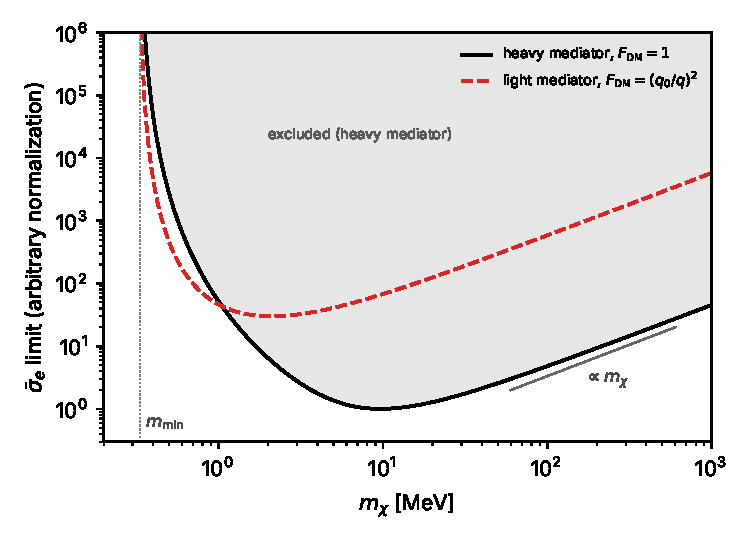
\includegraphics[width=0.72\linewidth]{figures/ch01/fig1_9.pdf}
  \caption{Schematic exclusion limits on $\sigmae$ for a silicon-like target. The threshold is the low-temperature gap $\Eg = \SI{1.17}{eV}$. The curves follow from \cref{eq:1.5-limscaling} with the standard-halo $\eta(\vmin)$ of \cref{sec:1.3} and a toy response: $S(q,\omega)$ flat between $\Eg$ and \SI{30}{eV}, multiplied by the Gaussian cutoff $\exp[-q^2/2(2q_0)^2]$ with $q_0 = \alpha m_e = \SI{3.73}{keV}$. Each curve has an arbitrary normalization (the light-mediator curve is shifted up for legibility). Both curves rise without bound at the threshold mass $m_{\mathrm{min}} = \SI{0.33}{MeV}$ (dotted) and grow as $m_\chi$ at large mass. The heavy-mediator curve ($\FDM = 1$) reaches its minimum at \SI{9.7}{MeV}, where the allowed momenta cover the cutoff; the light-mediator curve ($\FDM = (q_0/q)^2$), dominated by the smallest $q$, reaches its minimum at \SI{2.1}{MeV}. The shaded region is excluded by the heavy-mediator search.}
  \label{fig:1-exclusion}
\end{figure}

\paragraph{The low-mass edge.} Below $m_{\mathrm{min}} = 2E_{\mathrm{th}}/v_{\mathrm{max}}^2$ (\cref{eq:1.3-mmin}) no dark-matter particle in the halo can deposit $E_{\mathrm{th}}$, the integral in \cref{eq:1.5-limscaling} vanishes and the limit is infinite. Just above $m_{\mathrm{min}}$ only the fastest particles contribute, and $\eta$ grows from zero quadratically in the distance from the escape speed (\cref{eq:1.3-edge}): the curve falls steeply from a vertical wall. The position of the wall depends only on the threshold and on $v_{\mathrm{max}}$; a lower threshold moves it to lower mass in proportion (\cref{sec:1.3-edge}).

\paragraph{The heavy-mediator slope.} With $\FDM = 1$ the integrand of \cref{eq:1.5-limscaling} grows with $q$ through the factor $q\,\dd q$, and the maximum momentum transfer, $2m_\chi v_{\mathrm{max}}$, grows with $m_\chi$. It equals $q_0$ at \SI{0.70}{MeV} (\cref{sec:1.3}). The integral keeps growing until $2m_\chi v_{\mathrm{max}}$ passes the momenta of the valence electrons, a few $q_0$, which happens at masses around \SI{10}{MeV}; the curve falls over this whole range. Above it the integral is constant, $\mu_{\chi e} = m_e$, and only the factor $m_\chi$ remains: $\sigmae^{\mathrm{lim}} \propto m_\chi$, a line of slope one on logarithmic axes. The heavier dark matter is less numerous at fixed $\rho_\chi$.

\paragraph{The light-mediator slope.} With $\FDM = (q_0/q)^2$ the weight $(q_0/q)^4\,q\,\dd q$ favors the smallest momentum transfer that can deposit the threshold, $q \approx E_{\mathrm{th}}/v_{\mathrm{max}}$ (\cref{sec:1.3}). That momentum transfer is reachable as soon as $m_\chi$ is a few times $m_{\mathrm{min}}$, and the light-mediator curve turns over close to the edge, growing as $m_\chi$ from a few MeV upward. Because the rate comes from small $q$, the light-mediator limit is also the one most affected by screening (\cref{sec:4.4}) and by the low-energy end of the ionization yield.

As a result, the two curves are not related by a constant factor, and a limit quoted for one mediator cannot be rescaled to the other without the response. In the toy of \cref{fig:1-exclusion} the heavy-mediator limit at \SI{1}{MeV} stands a factor of 49 above its minimum at \SI{9.7}{MeV}, while the light-mediator limit is already within a factor of 1.5 of its minimum at \SI{2.1}{MeV}. A two-pair threshold would move both walls from 0.33 to \SI{1.36}{MeV}. Real exclusion plots add curves from several experiments and the benchmark cross-sections of thermal and freeze-in models (\cref{we:1-darkphoton}).

\subsection{Inputs of a limit}\label{sec:1.5-inputs}

Every exclusion curve combines measured inputs from the detector with theory inputs, and \cref{fig:1-chain} marks the boundary. The measured inputs belong to the detector: the exposure $M_{\mathrm{det}}t_{\mathrm{exp}}$, the threshold, the efficiency with which events pass the selection, the background and the observed count. Their errors are statistical or come from calibration, and experiments propagate them.

The theory inputs are the halo parameters, the particle-physics model and the response of the target. The halo parameters $\rho_\chi$, $v_0$ and $v_{\mathrm{esc}}$ are fixed by convention to the values of \cref{sec:1.2} so that experiments can be compared (\cref{app:A.8}); the limit scales as $1/\rho_\chi$, and $v_{\mathrm{esc}}$ moves the edge (\cref{sec:1.3-edge}). The particle physics enters only through $\FDM$, which is a definition of the model rather than an approximation (\cref{sec:1.4}). The target enters through $S(q,\omega)$ and through the conversion from $\omega$ to quanta, $N_{\mathrm{eh}}(\omega)$ for charge detectors. Both are computed, not measured, in the eV range that matters for light dark matter. Their errors are not statistical: they come from approximations, such as the treatment of exchange and correlation in the band structure, the neglect of screening or of phonons, or the step model of \cref{eq:1.5-step}. A longer exposure does not reduce them. Their effect on a limit follows from \cref{eq:1.5-limscaling}. A fractional error in $S(q,\omega)$ at the momentum transfers that dominate the integral moves the limit by the same fraction. An error in the gap or in the threshold energy moves the edge, $\delta\ln m_{\mathrm{min}} = \delta\ln E_{\mathrm{th}}$ (\cref{sec:1.3-edge}), and near the edge it changes the limit by a much larger factor, because $\eta$ varies steeply there. Together these errors make up the \emph{theory uncertainty} of a limit.

Two lines of argument start here: the signal chain and the theory uncertainty. The first follows the signal chain of \cref{fig:1-chain} from the response of the target to the measured signal: \crefrange{chap:2}{chap:7} build the response, and later chapters follow the deposit through the cascade to the sensor (\cref{chap:18,chap:20}). The second follows the theory uncertainty: each approximation, when it is introduced, comes with an estimate of its error, and \cref{chap:21} turns these estimates into uncertainties on exclusion limits.

\section*{Summary}

The event rate is an integral over a product of three factors, the halo, the coupling $|\tilde V(\vect q)|^2$ and the dynamic structure factor $S(\vect q,\omega)$ of the target, tied together by energy conservation (\cref{sec:1.1}). The particle physics and the condensed-matter physics therefore separate, and most of the book computes $S$. Gravity measures the density of dark matter but not its mass: a local density of a few tenths of a \si{GeV.cm^{-3}} (\cref{sec:1.2}) and a cosmological density $\Omega_{\mathrm{c}}h^2 = 0.120$ from the cosmic microwave background. The mass is open over some 90 decades, and the keV--GeV window is the range where the kinetic energy of halo dark matter, $\frac12 m_\chi v^2$ with $v \approx 10^{-3}$, matches the meV--eV excitations of solids. A thermal relic needs $\langle\sigma v\rangle \approx \SIrange{2e-26}{3e-26}{cm^3.s^{-1}}$, which below a few GeV requires a light mediator; freeze-in is the main alternative.

The local halo is described by the standard halo model (\cref{sec:1.2}): a truncated Maxwell--Boltzmann distribution with $\rho_\chi = \SI{0.3}{GeV.cm^{-3}}$, $v_0 = \SI{238}{km.s^{-1}}$ and $v_{\mathrm{esc}} = \SI{544}{km.s^{-1}}$, seen in the laboratory through the Earth's motion. The largest laboratory speed is $v_{\mathrm{max}} = \SI{794.5}{km.s^{-1}}$. The Earth's orbit modulates the rate annually, with a phase that reverses at $\vmin \approx \SI{211}{km.s^{-1}}$, and its rotation turns a crystal through the dark-matter wind once per sidereal day.

Kinematics (\cref{sec:1.3}) relates the momentum $q$ and energy $\omega$ given to the target through $\omega_{\vect{q}} = \vect q\cdot\vect v - q^2/2m_\chi - \Delta_\chi$, and every scattering rate contains $\eta(\vmin)$, the mean inverse speed above the minimum speed $\vmin$. A threshold $E_{\mathrm{th}}$ is reachable only above $m_{\mathrm{min}} = 2E_{\mathrm{th}}/v_{\mathrm{max}}^2$, \SI{0.33}{MeV} for the low-temperature silicon gap. Near $m_{\mathrm{min}}$ the rate vanishes quadratically with the tail of the halo. Electron transitions involve momentum transfers comparable to $q_0 = \alpha m_e = \SI{3.73}{keV}$, close to the shortest reciprocal-lattice vector of silicon, and free nuclear recoils deposit little energy for sub-GeV dark matter.

A mediator of mass $m_V$ produces the potential $\tilde V(q) = y_\chi y_e/(q^2 + m_V^2)$ (\cref{sec:1.4}). Its strength is quoted as the vacuum reference cross-section $\sigmae$ and its momentum dependence as $\FDM(q)$, equal to 1 for a heavy and $(q_0/q)^2$ for a light mediator. The dark photon is the standard example; bosonic dark matter can instead be absorbed, depositing $\omega \approx m_\phi$ at $q \approx 0$.

A detector counts electron--hole pairs (\SIrange{3.6}{3.75}{eV} each in silicon), phonons, quasiparticles (about \SI{0.36}{meV} per pair in bulk aluminum) or photons (\cref{sec:1.5}). The rate is linear in $\sigmae$ and $\rho_\chi$ and falls as $1/m_\chi$ well above threshold. With no events and no background the \SI{90}{\percent} upper limit is 2.3 expected events, and the cross-section limit improves in proportion to the exposure. Exclusion curves have a vertical edge at $m_{\mathrm{min}}$ and grow as $m_\chi$ at large mass. Their accuracy rests on the computed response of the target, which \crefrange{chap:2}{chap:7} develop. The errors of that computation, the theory uncertainty, do not shrink with exposure, and the book estimates them with each approximation it makes.
